\begin{align*}
    \polynomialQ{2}{X}{0} &= 0 \\
    \polynomialQ{2}{X}{1} &= 1 \\
    \polynomialQ{2}{X}{2} &= 30X^2 - 60X + 32 \\
    \polynomialQ{2}{X}{3} &= 150X^2 - 540X + 513 \\
    \polynomialQ{2}{X}{4} &= 420X^2 - 2160X + 2944 \\
    \polynomialQ{2}{X}{5} &= 900X^2 - 6000X + 10625 \\
    \polynomialQ{2}{X}{6} &= 1650X^2 - 13500X + 29376 \\
    \polynomialQ{2}{X}{7} &= 2730X^2 - 26460X + 68257 \\
    \polynomialQ{2}{X}{8} &= 4200X^2 - 47040X + 140288 \\
    \polynomialQ{2}{X}{9} &= 6120X^2 - 77760X + 263169 \\
    \polynomialQ{2}{X}{10} &= 8550X^2 - 121500X + 460000 \\
    \polynomialQ{2}{X}{11} &= 11550X^2 - 181500X + 760001 \\
    \polynomialQ{2}{X}{12} &= 15180X^2 - 261360X + 1199232 \\
    \polynomialQ{2}{X}{13} &= 19500X^2 - 365040X + 1821313 \\
    \polynomialQ{2}{X}{14} &= 24570X^2 - 496860X + 2678144 \\
    \polynomialQ{2}{X}{15} &= 30450X^2 - 661500X + 3830625 \\
    \polynomialQ{2}{X}{16} &= 37200X^2 - 864000X + 5349376 \\
    \polynomialQ{2}{X}{17} &= 44880X^2 - 1109760X + 7315457 \\
    \polynomialQ{2}{X}{18} &= 53550X^2 - 1404540X + 9821088 \\
    \polynomialQ{2}{X}{19} &= 63270X^2 - 1754460X + 12970369 \\
    \polynomialQ{2}{X}{20} &= 74100X^2 - 2166000X + 16880000
\end{align*}
\begin{figure}[H]
    \centering
    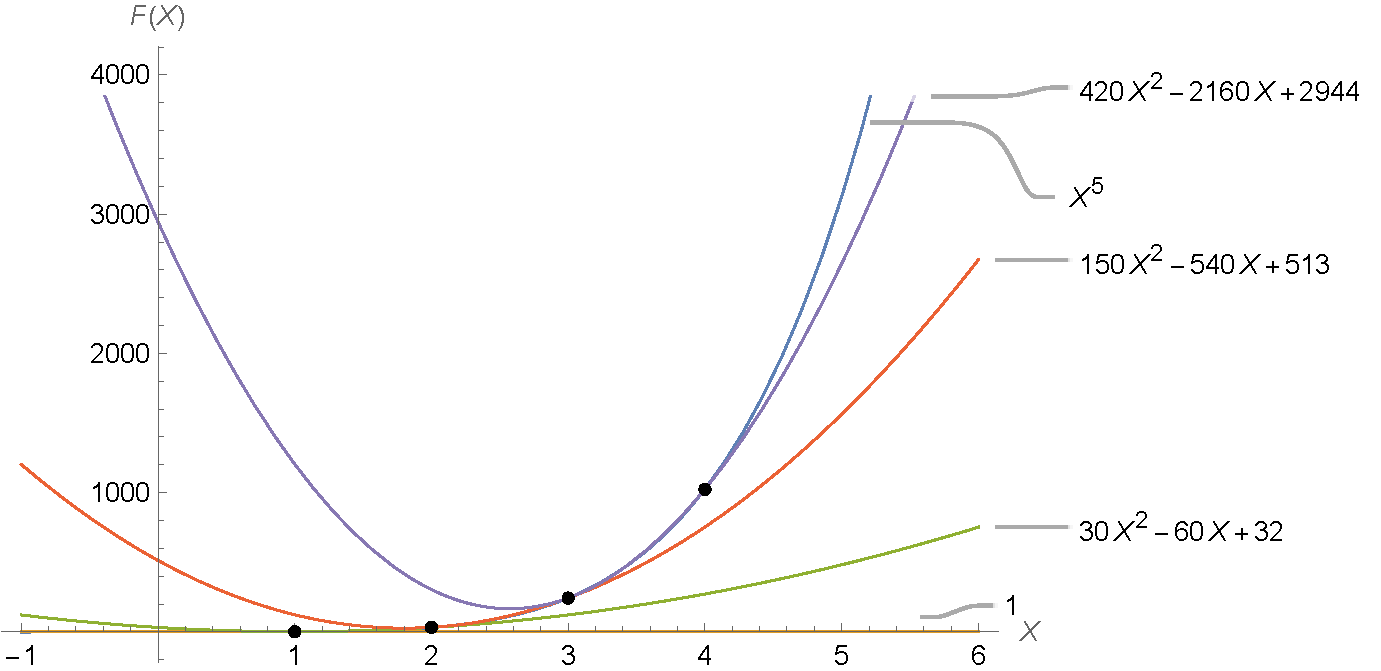
\includegraphics[width=1\textwidth]{sections/images/04_fifth_power_with_q_1_n_k}
    ~\caption{Polynomials Q(2, n, k)}\label{fig:figure4}
\end{figure}
